\documentclass[../p023main.tex]{subfiles}
\graphicspath{{\subfix{../figures/}}}

\begin{document}

\chapter{Conservation Laws in Spacetime}
\section{Spacetime}
The Lorentz transformation has shown us how space and time transform in such a way that they cannot be considered separately.
This leads naturally into the notion of spacetime, the geometry of which is slightly different from the Euclidean geometries we're used to seeing in the world.

A visual will be useful to us in understanding this ``pseudo-Euclidean'' geometry, which we'll call Minkowski space (after its inventor).
Of course, we'd need to work in four dimensions to fully do it justice, but we can communicate the key ideas by working with just one or two spatial dimensions.

Let's start with two.
We might model ``(1+2)-dimensional'' spacetime by putting two spatial dimensions in the $xy$-plane and one temporal dimension on the vertical axis.
If we consider the paths of all possible beams of light passing through the origin $(0,0,0)$, we get the double-cone below.
All massive objects travel more slowly than the speed of light and so are trapped within this ``light cone''.
\begin{center}
    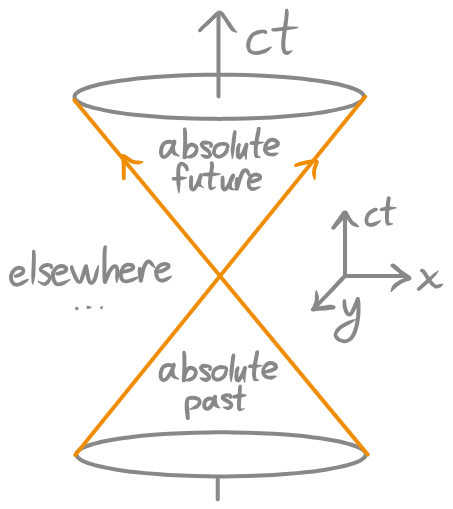
\includegraphics[width=0.35\textwidth]{lightCone.png}
\end{center}
Note that from here on out we will refer to time as $ct$ rather than just $t$.
There's nothing fundamental going on here, this is just a mathematical convenience---for example, we'll soon find some use in time having the same units as space.

Suppose an event $E$ occurs at the origin.
The bottom cone, called the \textit[absolute past] of $E$, contains all events which could possible have influenced $E$ in any way.
(Events outside the cone would need their influence to travel faster than the speed of light, which is impossible.)
Similarly, the top cone, called the \textit{absolute future} of $E$, contains all events which $E$ could possibly influence.

The above is true for any reference frame.
If an event happens in the absolute past in one frame, it also happens in the past for all others.
Outside the double-cone, however, all bets are off---here a past event in one frame could be a future event in another.
This region is often simply called \textit{elsewhere}.

To make this a little more mathematical, we can draw a rough analogy to something more familiar.
In Euclidean space, rotations leave distances unchanged.
If we take two points and rotate them about the origin, the ``before'' distance is the same as the ``after'' distance.
Therefore, we say that the quantity
\[ (\Delta r)^2 = (\Delta x)^2 + (\Delta y)^2 + (\Delta z)^2 \]
is invariant under rotations.
(Notice how this looks like the equation for a sphere or, in 2D, a circle!)

It's useful to think of spacetime has having a geometry that has werid rules for rotations involving both space and time.
Just as rotations in Euclidean space leave circles unaffected, ``rotations'' in spacetime leave hyperbolas unaffected.\footnote{A good Desmos visual can be found here: https://www.desmos.com/calculator/r75hsbvmbj}
As a result, an event occurs on the same hyperbola in all reference frames.
This means the quantity $s^2 = -(ct)^2 + x^2 + y^2 + z^2$ is unvariant under the Lorentz transformation!

We can use this fact to define the spacetime interval, a sort of absolute ``distance'' between events that is independent of reference frames:
\[ (\Delta s)^2 \equiv -(c \Delta t)^2 + (\Delta x)^2 + (\Delta y)^2 + (\Delta z)^2. \]
An interesting characteristic of $(\Delta s)^2$ is that it can be positive, zero, or negative!
Each corresponds to a different type of separation between events.
\begin{itemize}
    \item If $(\Delta s)^2 > 0$ then we have a spacelike interval---there is more separation in space than in time.
    Here we can always find a reference frame in which the events are simultaneous; the spatial separation in this frame is known as the \textit{proper length} between the events.
    \item If $(\Delta s)^2 < 0$ then we have a timelike interval---there is more separation in time than in space.
    Here we can always find a reference frame in which the events occur in the same place; the temporal separation in this frame is known as the \textit{proper time} between the events.
    \item If $(\Delta s)^2 = 0$ then we have a null interval.
    This corresponds to events that occur along a light ray.
\end{itemize}
Events that are separated by a timelike or null interval are in each others' absolute past and futures.
For spacelike intervals, the order of events is relative.

\begin{summary}
    Lorentz transformations can be thought of as rotations in a space built upon hyperbolas rather than circles.
    This hyperbolic geometry gives us the spacetime interval
    \[ (\Delta s)^2 \equiv -(c \Delta t)^2 + (\Delta x)^2 + (\Delta y)^2 + (\Delta z)^2, \]
    which can be interpreted as a sort of ``distance'' between events in spacetime.
    The value of a spacetime interval is not affected by Lorentz transformations, and it gives us information about whether the separation between the events is mostly spatial or temporal (or both).
\end{summary}


\section{Momentum}
Armed with a better understanding of spacetime, we can now re-examine some fundamental concepts from Newtonian mechanics.
To do this, we must define the \textit{four-vector}---the spacetime analog to Euclidean vectors.

It may not be surprising that four-vectors are described by four numbers:
\[ A_\mu = (A_0, A_x, A_y, A_z). \]
Four-vectors must transform according to the Lorentz transformation:
\begin{align*}
    A_0' &= \gamma \left( A_0 - \frac{VA_x}{c} \right) \\
    A_x' &= \gamma \left( A_x - \frac{VA_0}{c} \right) \\
    A_y' &= A_y \\
    A_z' &= A_z
\end{align*}
So it follows that, for any four-vector, the quantity
\[ -A_0^2 + A_x^2 + A_y^2 + A_z^2 \]
is invariant under the Lorentz transformation.
(This makes it a \textit{four=-scalar}, a number whose value does not change after a Lorentz transformation.)

Now, consider a particle floating around in spacetime.
The simplest four-vector describing the particle is the four-position
\[ z_\mu = (ct, x, y, z). \]
We can define the four-momentum as
\[ p_\mu \equiv m \frac{dx\mu}{d\tau}; \]
where $m$ is the mass of the particle and $\tau$ is its proper time---that is, the time read by a clock moving alongside the particle.
The quantity $\frac{dx\mu}{d\tau}$ is called the four-velocity, and we differentiate it with respect to $\tau$ because it is a four-scalar.
(Otherwise, it would give us something different in each reference frame!)

We can expand our expression a bit:
\[ p_\mu = m \left( c \frac{dt}{d\tau}, \frac{dx}{d\tau}, \frac{dy}{d\tau}, \frac{dz}{d\tau} \right). \]
Due to time dilation,
\[ \frac{dt}{d\tau} = \frac{1}{\sqrt{1 - \left( \frac{v}{c} \right)^2}}, \]
where $v$ is the speed at which the particle is observed to move.
We'll call this quantity $\gamma$.
(Notice how this $\gamma$ is subtly different from the one we defined previously, in which $V$ was a relative speed between reference frames; we can reconcile this by interpreting $v$ as the speed between our frame and the particle's rest frame.)

Now, by the chain rule,
\[ \frac{dx}{d\tau} = \frac{dx}{dt} \frac{dt}{d\tau} = \gamma v_x, \]
where $v_x$ is the $x$-component of the particle's observed velocity.
Therefore,
\[ p_\mu = (\gamma mc, \gamma mv_x, \gamma mv_y, \gamma mv_z) = (\gamma mc, \gamma m\mbf{v}). \]
The spatial component of this four-vector is the relativistic momentum!
That is,
\[ \mbf{p} = \gamma m\mbf{v}. \]
Notice that at low speeds $\gamma \approx 1$, and we recover the classical $\mbf{p} = m\mbf{v}$.

It has been shown, through, experiment that this momentum is conserved in collisions.
It is also easy to show, using the Lorentz transformation, that if momentum is conserved in one frame then it is conserved in all other frames.
So this quantity has the universal importance we seek!

\begin{summary}
    Four-vectors are objects that transform according to the Lorentz transformation. If a four-vector is specified by the components $A_\mu = (A_0, A_x, A_y, A_z)$, then the quantity
    \[ -A_0^2 + A_x^2 + A_y^2 + A_z^2 \]
    is invariant under the Lorentz transformation.

    The most basic four-vector is the four-position $x_\mu = (ct, x, y, z)$. Another is the four-momentum, defined by
    \[ p_\mu \equiv \frac{dx_\mu}{d\tau} = (\gamma mc, \gamma m\mathbf{v}). \]
    The spatial $\mathbf{p} = \gamma m \mathbf{v}$ is the relativistic momentum, and it is conserved in collisions.
\end{summary}

\section{Energy}
The relativistic momentum $\mbf{p}$ that we found in the previous section only encompasses the spatial components of the four-momentum.
What about the temporal component $p_0$?
What does it represent?

Notice that $p_0$ is a scalar that is conserved.
The obvious candidate is energy.
The unit discrepancy is no problem---we can just multiply by $c$ to get units of energy, just like wedid when formulating spacetime.

To see if this makes sense, consider the series expansion of $p_0c$:
\begin{align*}
    p_0c &= \frac{mc^2}{\sqrt{ 1 - \left( \frac{v}{c} \right)^2 }} \\
    &= mc^2 \left( 1 + \frac{1}{2} \left( \frac{v}{c} \right)^2 + \cdots \right) \\
    &= mc^2+ \frac{1}{2}mv^2 + \cdots
\end{align*}
We can immediately see that the object's energy increases as it moves faster, which checks out.
This is just the idea of kinetic energy.
Specifically, the kinetic energy of the object is given by all the velocity-dependent terms in $p_0c$; that is,
\[ K = \gamma mc^2 - mc^2 = (\gamma - 1)mc^2. \]
Also notice that, in the nonrelativistic limit $v \ll c$, this kinetic energy is simply $\frac{1}{2}mv^2$---which is exactly what we'd expect from Newtonian mechanics!

There's this other term, though, that's completely independent of the object's speed, or even its position in space.
This quantity,
\[ E_0 = mc^2, \]
is called the \textit{mass energy} (or \textit{rest energy}) of the object.
It is the energy that the object has just by existing!

So $E = p_0c$ is the energy of an object.
We can now write the four-momentum as
\[ p_\mu = (\gamma mc^2, \gamma m\mbf{v}) = \left( \frac{E}{c}, \mbf{p} \right). \]
The invariant associated with this four-vector is
\[ -(\gamma mc^2)^2 + (\gamma mv)^2 = \left( \frac{E}{c} \right)^2 + p^2. \]
Manipulating the left-hand side gives
\[ -(mc)^2 = \left( \frac{E}{c} \right)^2 + p^2 \]
or, alternatively,
\[ E^2 = (pc)^2 + (mc^2)^2. \]
This is another very important Lorentz invariant, this time showing that energy and momentum are fundamentally related!
It's also true for all objects, including massless ones.
Thus the energy and momentum of a photon are related by
\[ E = pc. \]
As one final tidbit, we'll give a particularly interesting consequence of these conservation laws.

Consider the decay of a particle of mass $M$ into two identical particles, each of mass $m$.
By conservation of momentum, the resulting particles fly off in opposite directions with the same speed $v$; by conservation of energy, though,
\[ Mc^2 = 2 \gamma mc^2 \implies M = \gamma \cdot 2m. \]
Since $\gamma \neq 1$, mass has not been conserved!
Specifically, some of the original mass energy has been converted into kinetic energy, so $M > 2m$.
Yet another wildly unintuitive result from special relativity, that conservation of mass does not exist.

\begin{summary}
    The temporal component of an objet's four-momentum represents its total energy,
    \[ E = \gamma mc^2. \]
    This energy has two components: the mass energy $E_0 = mc^2$ and the kinetic energy $K = (\gamma - 1)mc^2$.
    This leads to a new Lorentz invariant,
    \[ E^2 = (pc)^2 + (mc^2)^2, \]
    which applies to all particles, including massless ones.

    Together, conservation of energy and momentum leads to the surprising fact that mass is not necessarily conserved in collisions.
\end{summary}

    
\end{document}